\documentclass[10pt,oneside]{report}

\usepackage{indentfirst}
\usepackage{placeins}

% The preamble contains definitions and settings
%%% Preamble
\usepackage{amsmath}
\usepackage{amssymb}
\usepackage{latexsym}
\usepackage{graphicx}


%%%
%%% Bibliography
%%%
\usepackage[backend=bibtex8, citestyle=numeric, bibstyle=authortitle]{biblatex}
\bibliography{/Users/rh/refs/preamble.bib,
  /Users/rh/refs/ieee-1471.bib, /Users/rh/refs/cs.bib, /Users/rh/refs/arch.bib}

%%% 
%%% Definitions
%%%
\newcommand{\Fillin}[1]{\textcolor{Red}{$<$#1$>$}}
\newcommand{\HRule}{\rule{\linewidth}{0.5mm}}
\newcommand{\Optional}{\textcolor{Gray}{\textsf(optional)}}
\newcommand{\angles}[1]{$\langle$#1$\rangle$}
\newcommand{\must}[1]{\textcolor{NavyBlue}{$\star$ #1}}
\newcommand{\note}[1]{\small\textsc{note: }\textit{#1}}
\newcommand{\should}[1]{\textcolor{Plum}{$\Box$ #1}}
\newcommand{\std}[1]{\textcolor{Maroon}{ISO/IEC/IEEE~42010,~#1}}
\newcommand{\tbd}[1]{\noindent\textcolor{Red}{\textbf{TBD: }{\textsf{#1}}}}
\newcommand{\working}[1]{\noindent\textcolor{CadetBlue}{\textsf{#1}}}

% \renewcommand{\thesection}{\Alph{section}}
% \renewcommand{\thesubsection}{\alph{subsection}}
% \renewcommand{\thesubsubsection}{\roman{subsection}.}

\parindent 0cm
\parskip 0.3cm

% \topmargin 0.2cm
% \oddsidemargin 1cm
% \evensidemargin 0.5cm
% \textwidth 14cm
% \textheight 20cm
% \pagestyle{fancy}

%%%  Prettier Tables
% \usepackage{booktabs}
%%%  Diagrams
% \usepackage[all]{xy}


%%%
%%%  Colors
%%%
\usepackage{color}
\usepackage[usenames,dvipsnames]{xcolor} % see: http://en.wikibooks.org/wiki/LaTeX/Colors


%%% Fonts
%\usepackage[charter]{mathdesign}
%\usepackage{arev}
%\usepackage{ccfonts,eulervm} \usepackage[T1]{fontenc}
%\usepackage{cmbright}
%\usepackage{concrete}
%\usepackage{kmath,kerkis}
%\usepackage{mathpazo}
%\usepackage{mathptmx}
\usepackage{newcent}
%\usepackage{palatino}
%\usepackage{pxfonts}
%%% end Fonts


%%% Index
%%% \makeindex


%%% Make this last package (always load after biblatex):
\usepackage[pdfstartview=FitH,colorlinks=true,citecolor=ForestGreen,linkcolor=NavyBlue]{hyperref}

%%% end Preamble



\begin{document}

\begin{titlepage}

\centering


\includegraphics[width=7cm]{Wits-logo1.jpg}

\vskip 0.1cm

\center 

\textsc{\LARGE University of the Witwatersrand}\\[0.4cm] 

\textsc{\Large Architecture Description of \\ 
    Layered Architecture for \\[0.1cm] 
    HealFolio} \\[0.4cm] 

\begin{minipage}{0.4\textwidth}

\begin{center} \large

\textbf{Team Name:} \\[0.2cm]

\textsc{Level Seven Crew} \\[0.2cm]

\end{center}

\begin{center} \large

\textbf{Product Name:} \\[0.2cm]

\textsc{HealFolio} \\[0.7cm]

\end{center}

\begin{flushleft} \large

\textbf{Team Members:} \\[0.2cm]

Jan \textsc{Badenhorst} \\
Adam \textsc{Lerumo} \\
Tumbone \textsc{Asukile} \\
Daniel da \textsc{Silva} \\

\end{flushleft}

\end{minipage} \\[0.5cm]

\begin{minipage}{0.4\textwidth}

\begin{flushright} \large

\textbf{Senior Lecturer:} \\[0.2cm]

Dr. Terence van \textsc{Zyl} \\

\end{flushright}

\end{minipage} \\[0.5cm]

{\large September 12, 2016} 
    
\end{titlepage}

\newpage
%%%%%%%%%%
\tableofcontents
% \listoffigures
% \listoftables
%%%%%%%%%%

%%%
%%% Change page number for main body of text
%%%
\pagenumbering{arabic}

\setlength\parindent{24pt}

%%%%%%%%%%
\chapter{Introduction}\label{ad:info}
%%%%%%%%%%

This chapter describes introductory information items of the Architecture Description (AD), including identifying and supplementary information.

%%%%%%%%%%
\section{Identifying information}\label{ad:idinfo}
%%%%%%%%%%

\begin{itemize}
\item The architecture being expressed is an Layered Architecture.
\item The system of interest is HealFolio, an individual applications for which this is an architecture description.
\end{itemize}

Following ISO/IEC/IEEE 42010, \textit{system} (or \textit{system-of-interest}) is a shorthand for any number of things including man-made systems, software products and services, and software-intensive systems including ``individual applications, systems in the traditional sense, subsystems, systems of systems, product lines, product families, whole enterprises, and other aggregations of interest''. \std{4.2}

%%%%%%%%%%
\section{Supplementary information}\label{ad:supinfo}
%%%%%%%%%%

\subsection{Date of issue and status}

\begin{itemize}
\item This project was started on the 24 of July 2016.
\end{itemize}

\subsection{Authors}

\begin{itemize}
\item Adam Lerumo - Product owner
\item Tumbone Asukile - Developer
\item Daniel da Silva - Developer
\item Jan Badenhorst - Scrum Master
\end{itemize}

\subsection{Reviewers}

\begin{itemize}
\item Dr. Terence van Zyl - Senior Lecturer and intellectual guide.
\end{itemize}

\subsection{Scope}

The team will be designing software (HealFolio) aimed at improving service delivery for all types of medical practitioners; specifically the filing system currently used by medical practitioners. This software will provide doctors with easier access to patient records and provide more security. It will also help them make more accurate diagnoses, provide better prescriptions and more as the software is further developed.

\subsection{Context}


The software to be implemented will operate in the medical industry, predominantly among General Practitioners (GP's). The issues in this sector include things such as (but not limited to):

\begin{itemize}

\item Patient record sharing across many different practices.

\item Security in the use of medical aid for visits to GP's and other practitioners.

\item Patient reaction to prescribed medications.

\end{itemize}

The above list provides a brief outline of the core issues to be addressed by the project, more issues may be identified as the project progresses.

\subsection{Overview}

The Layered Architecture pattern the is being used in HealFolio, otherwise known as the n-tier architecture pattern. This pattern is the standard for most Java EE applications and therefore is widely known by most architects, designers, and developers. The layered architecture pattern closely matches the traditional IT communication and organizational structures found in most companies, making it a natural choice for most business application development efforts.

\begin{figure}[h!]
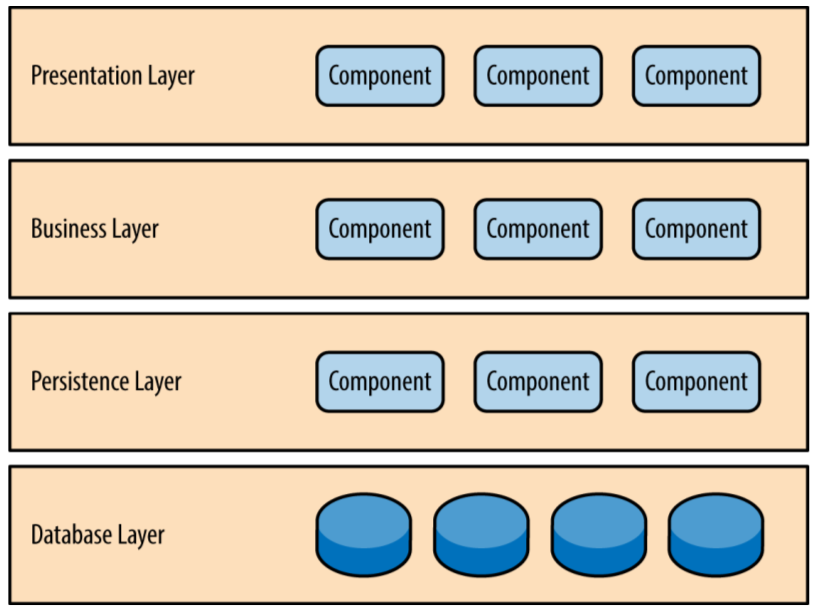
\includegraphics[width=15cm]{Layered-architecture-pattern.png}
\caption{Layered Architecture Pattern}
\label{Layered Architecture Pattern}
\end{figure}

This project is leaning toward the Microservices Architecture pattern. There are several common core concepts that apply to this architecture pattern. The first of these concepts is the notion of separately deployed units. Each component of the microservices architecture is deployed as a separate unit, allowing for easier deployment through an effective and streamlined delivery pipeline, increased scalability, and a high degree of application and component decoupling within your application. Perhaps the most important concept to understand with this pattern is the notion of a service component. Rather than think about services within a microservices architecture, it is better to think about service components, which can vary in granularity from a single module to a large portion of the application. Service components contain one or more modules (e.g., Java classes) that represent either single-purpose function (e.g., viewing information for a specific patient) or an independent portion of a our application (e.g., signing up for the service).

\begin{figure}[h!]
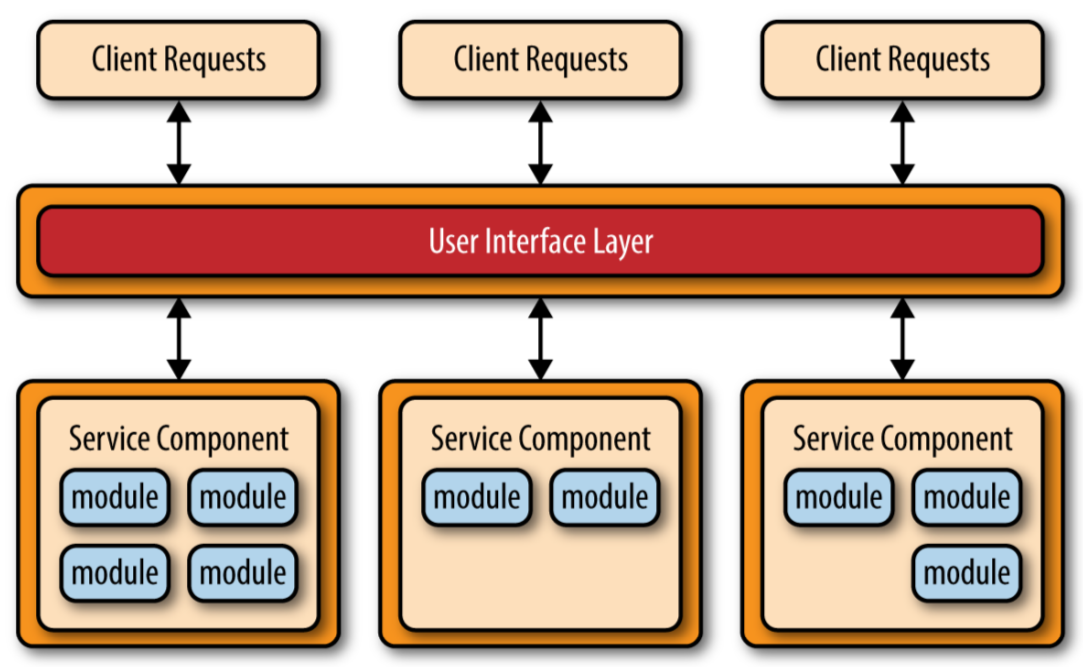
\includegraphics[width=15cm]{Basic-Microservices-architecture-pattern.png}
\caption{Basic Microservices architecture pattern}
\label{Basic Microservices architecture pattern}
\end{figure}

%%%%%%%%%%
\subsection{Architecture evaluations}
%%%%%%%%%%

Components within the layered architecture pattern are organized into horizontal layers, each layer performing a specific role within the application (e.g., presentation logic or business logic). Although the layered architecture pattern does not specify the number and types of layers that must exist in the pattern, most layered architectures consist of four standard layers: presentation, business, persistence, and database. In the case of our application so far the business layer and persistence layer are combined into a single business layer (a controller), particularly when the persistence logic is embedded within the business layer components. Thus our small application has only three layers.

Each layer of the layered architecture pattern has a specific role and responsibility within the application. The presentation layer is responsible for handling all user interface and browser communication logic, whereas as the business layer is responsible for executing specific business rules associated with the request and retrieving of information. Each layer in the architecture forms an abstraction around the work that needs to be done to satisfy a particular business request. For example, the presentation layer doesn’t need to know or worry about how to get customer data; it only needs to display that information on a screen in particular format. The business layer doesn’t need to be concerned about how to format patient data for display on a screen it needs to get the data from the database layer, perform business logic against the data (e.g., finding the diagnostic history of certain patients), and pass that information up to the presentation layer. 

One of the powerful features of the layered architecture pattern is the separation of concerns among components. Components within a specific layer deal only with logic that pertains to that layer. For example, components in the presentation layer deal only with presentation logic, whereas components residing in the business layer deal only with business logic. This type of component classification makes it easy to build effective roles and responsibility models into our architecture, and also makes it easy to develop, test, govern, and maintain applications using this architecture pattern due to well-defined component interfaces and limited component scope. 

%%%%%%%%%%
\subsection{Rationale for key decisions}
%%%%%%%%%%

The layered architecture pattern is a solid general-purpose pattern, making it a good starting point for most applications, particularly when you are not sure what architecture pattern is best suited for your application. However, there are a couple of things to consider from an architecture standpoint when choosing this pattern.

The first thing to watch out for is what is known as the architecture sinkhole anti-pattern. This anti-pattern describes the situation where requests flow through multiple layers of the architecture as simple pass-through processing with little or no logic performed within each layer. Every layered architecture will have at least some scenarios that fall into the architecture sinkhole anti-pattern. The key, however, is to analyze the percentage of requests that fall into this category. If one finds a majority of requests are simple pass-through processing, you might want to consider making some of the architecture layers open (meaning requests are allowed to bypass this open layer and go directly to the layer below it), keeping in mind that it will be more difficult to control change due to the lack of layer isolation.

Another consideration with the layered architecture pattern is that it tends to lend itself toward monolithic applications, even if you split the presentation layer and business layers into separate deploy-able units. While this may not be a concern for some applications, it does pose some potential issues in terms of deployment, general robustness and reliability, performance, and scalability.


%%%%%%%%%%
\chapter{Stakeholders and concerns}\label{sec:snc}
%%%%%%%%%%

This chapter contains information items for stakeholders of the 
architecture, the stakeholders' concerns for that architecture, and
the trace-ability of concerns to stakeholders. See also:~\std{5.3}

%%%%%%%%%%
\section{Stakeholders}\label{ad:stakeholders}
%%%%%%%%%%

A stakeholder is an individual, team, or organization with interests in, or concerns related to, the system-to-be. Generally, the system-to-be has several types of stakeholders: customers, end users, business analysts, systems architects and developers, testing and quality assurance engineers, project managers, the future maintenance organization, owners of other systems that will interact with the system-to-be.
 
 \begin{itemize}

\item \textbf{Customers and end users}
\begin{itemize}
\item The application will interact with people is the medical field, private practices, where doctors would be able to use relevant information from not only their past experience but a collective of as many practitioners that use the application. Where previous they had a to look a hard copy of patient and similar cases that would might be overlooked or very time consuming will now be able to call various report to there device from a vast database. The doctors and receptionists will be the users and operators of the application.
\end{itemize}
\item \textbf{Systems architects and developers}
\begin{itemize}
\item The team Level Seven Crew the acquirers, owners, developers, builders and testers of the application HealFolio. 
\item Dr. Terence van Zyl is a person of interest and will be evaluating as well as consult on the progress the team makes.
\end{itemize}
\end{itemize}

%%%%%%%%%%
\section{Concerns}\label{ad:concerns}
%%%%%%%%%%

\begin{itemize}
\item \textbf{What are the purpose(s) of the system-of-interest?} \\
Making referencing of information that would be otherwise too much of an ordeal, therefore streamlining the service giving by medical practitioners.
\item \textbf{What is the suitability of the architecture for achieving the system-of-interest's purpose(s)?} \\
Layered Architecture
\item \textbf{How feasible is it to construct and deploy the system-of-interest?} \\
With the opens source tools available, the direction of the course instructor and the time allocated makes tackling this project possible.
\item \textbf{What are the potential risks and impacts of the system-of-interest to its stakeholders throughout its life cycle?} \\
The sharing or leakage of confidential information can be an issue that has to addressed continuously thought-out the development and improvement of the application. The stakeholders might feel sharing diagnosis would be violating doctor patient privileges, and this needs to be pressed that security is key the application's development. 
\item \textbf{How is the system-of-interest to be maintained and evolved?} \\
With an eye on future the application will start of as a layered architecture and keeping in mind to migrate the application toward micro-services architecture with future improvement and growth.
\end{itemize}

%%%%%%%%%%
\section{Concern--Stakeholder Trace-ability}
%%%%%%%%%%

\subsection{List of concerns:}

\begin{enumerate}
\item \textbf{Concern 1} - Sharing or leakage of confidential information
\item \textbf{Concern 2} - Doctor patient confidentiality. 
\item \textbf{Concern 3} - Future growth and expansion. 
\end{enumerate}

\subsection{List of Stakeholders}

\begin{enumerate}
\item \textbf{Stakeholder 1} - Medical Practitioners
\item \textbf{Stakeholder 2} - Team Level Seven Crew 
\item \textbf{Stakeholder 3} - Lecturer 
\end{enumerate}

\begin{table}[h]
\caption{Showing association of stakeholders to concerns in an AD}\label{stakeholders concerns}
\begin{tabular}{ l | c | c | c | c }
& \textsf{Stakeholder~1} & \textsf{Stakeholder~2} & \textsf{Stakeholder~3} & \\
\hline
\textsf{Concern~1} & \textbf{x} & \textbf{x} & - & \\
\textsf{Concern~2} & \textbf{x} & \textbf{x} & \textbf{x} & \\
\textsf{Concern~3} &  &  & \textbf{x} & \\
\hline
\end{tabular}
\end{table}

%%%%%%%%%%
\chapter{Viewpoints}\label{ad:vps}
%%%%%%%%%%

\textbf{Definition}: A viewpoint is a collection of patterns, templates, and conventions for constructing one type of view. It defines the stakeholders whose concerns are reflected in the viewpoint and the guidelines, principles, and template models for constructing its views.

%%%%%%%%%%
\section{Architecture Model}\label{mk:list}
%%%%%%%%%%

A model is a complete, basic, and simplified description of software architecture which is composed of multiple views from a particular perspective or viewpoint.

A view is a representation of an entire system from the perspective of a related set of concerns. It is used to describe the system from the viewpoint of different stakeholders such as end-users, developers, project managers, and testers.


%%%%%%%%%%
\subsection{4+1 Model}\label{vp:mk}
%%%%%%%%%%

The 4+1 View Model was designed by Philippe Kruchten to describe the architecture of a software-intensive system based on the use of multiple and concurrent views. It is a multiple view model that addresses different features and concerns of the system. It standardizes the software design documents and makes the design easy to understand by all stakeholders.

It is an architecture verification method for studying and documenting software architecture design and covers all the aspects of software architecture for all stakeholders. It provides four essential views:

\begin{figure}[h!]
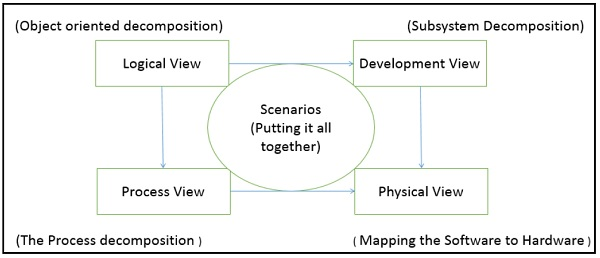
\includegraphics[width=15cm]{four-plus-one-view-model.jpg}
\caption{4+1 Model}
\label{Basic Micro-services architecture pattern}
\end{figure}

\begin{itemize}
\item \textbf{The logical view or conceptual view} - It describes the object model of the design.
\item \textbf{The process view} - It describes the activities of the system, captures the concurrency and synchronization aspects of the design.
\item \textbf{The physical view} - It describes the mapping of software onto hardware and reflects its distributed aspect.
\item \textbf{The development view} - It describes the static organization or structure of the software in its development of environment.
\end{itemize}

This view model can be extended by adding one more view called scenario view or use case view for end-users or customers of software systems. It is coherent with other four views and are utilized to illustrate the architecture serving as “plus one” view, (4+1) view model. The following figure describes the software architecture using five concurrent views (4+1) model.

%%% include Viewpoint Template here:
%%% Version 2.1b %%%

%%%%%%%%%%
\section{\Fillin{Viewpoint Name}}\label{vp:template}
%%%%%%%%%%

\must{Provide the name for the viewpoint.}

If there are any synonyms or other common names by which this viewpoint is
known or used, record them here.


%%%%%%%%%%
\section{Overview} 
%%%%%%%%%%

Provide an abstract or brief overview of the viewpoint. 

Describe the viewpoint's key features.


%%%%%%%%%%
\section{Concerns and stakeholders} 
%%%%%%%%%%

Architects looking for an architecture viewpoint suitable for their
purposes often use the identified concerns and typical stakeholders to
guide them in their search.  Therefore it is important (and required
by the Standard) to document the concerns and stakeholders for which a
viewpoint is intended.

%%%%%%%%%%
\subsection{Concerns}\label{vp:concerns}
%%%%%%%%%%

\must{Provide a listing of architecture-relevant concerns to be framed by
this architecture viewpoint per \std{7a}.}

Describe each concern.

Concerns name ``areas of interest'' in a system.

\note{Following ISO/IEC/IEEE 42010, \textbf{system} is a shorthand for
  any number of things including man-made systems, software products
  and services, and software-intensive systems such as ``individual
  applications, systems in the traditional sense, subsystems, systems
  of systems, product lines, product families, whole enterprises, and
  other aggregations of interest''.}

Concerns may be very general (e.g., \textit{Reliability}) or quite
specific (\textit{e.g., How does the system handle network latency?}).
  
Concerns identified in this section are critical information for an
architect because they help her decide when this viewpoint will be
useful.

When used in an architecture description, the viewpoint becomes a
``contract'' between the architect and stakeholders that these
concerns will be addressed in the view resulting from this viewpoint.

It can be helpful to express concerns \emph{in the form of questions}
that views resulting from that viewpoint will be able to answer. E.g.,
\begin{itemize}
\item \textit{How does the system manage faults?}
\item \textit{What services does the system provide?}
\end{itemize}

\note{``In the form of a question'' is inspired by the television quiz
  show, \textit{Jeopardy!}}
 
\std{5.3} contains a candidate list of concerns that must be considered
when producing an architecture description. These can be considered
here for their relevance to the viewpoint being specified:
\begin{itemize}
\item What are the purpose(s) of the system-of-interest?
\item What is the suitability of the architecture for achieving the
  system-of-interest's purpose(s)?
\item How feasible is it to construct and deploy the
  system-of-interest?
\item What are the potential risks and impacts of the
  system-of-interest to its stakeholders throughout its life cycle?
\item How is the system-of-interest to be maintained and evolved?
\end{itemize}

See also: \std{4.2.3}.

%%%%%%%%%%
\subsection{Typical stakeholders} 
%%%%%%%%%%

\must{Provide a listing of the typical stakeholders of a system who
  are in the potential audience for views of this kind, per \std{7b}.}

Typical stakeholders would include those likely to read such views
and/or those who need to use the results of this view for another
task.

Stakeholders to consider include:
\begin{itemize}
\item users of a system; 
\item operators of a system; 
\item acquirers of a system;
\item owners of a system; 
\item suppliers of a system; 
\item developers of a system; 
\item builders of a system; 
\item maintainers of a system.
\end{itemize}

%%%%%%%%%%
\subsection{``Anti-concerns'' \Optional} 
%%%%%%%%%%

It may be helpful to architects and stakeholders to
document the kinds of issues for which this viewpoint is \emph{not
  appropriate or not particularly useful}.

Identifying the ``anti-concerns'' of a given notation or approach may
be a good antidote for certain overly used models and notations.

% \tbd{Examples!}



%%%%%%%%%%
\section{Model kinds+}\label{mk:list}
%%%%%%%%%%

\must{Identify each model kind used in the viewpoint per \std{7c}.}

In the Standard, each architecture view consists of multiple
architecture models. Each model is governed by a \textit{model kind}
which establishes the notations, conventions and rules for models of
that type.  See: \std{4.2.5, 5.5 and 5.6}.

Repeat the next section for each model kind listed here the viewpoint
being specified.


%%%%%%%%%%
\section{\Fillin{Model Kind Name}}\label{vp:mk}
%%%%%%%%%%

\must{Identify the model kind.}


%%%%%%%%%%
\subsection{\Fillin{Model Kind Name} conventions} 
%%%%%%%%%%

\must{Describe the conventions for models of this kind.}

Conventions include languages, notations, modeling techniques,
analytical methods and other operations. These are key modeling
resources that the model kind makes available to architects and
determine the vocabularies for constructing models of the kind and
therefore, how those models are interpreted and used.

It can be useful to separate these conventions into a \emph{language
  part}: in terms of a metamodel or specification of notation to be
used and a \emph{process part}: to describe modeling techniques used
to create the models and methods which can be used on the models that
result.  These include operations on models of the model kind.

The remainder of this section focuses on the language part. The next
section focuses on the process part.

The Standard does not prescribe \emph{how} modeling conventions are to
be documented.  The conventions could be defined:
\begin{description}
\item[I)] by reference to an existing notation or language (such as
  SADT, UML or an architecture description language such as ArchiMate
  or SysML) or to an existing technique (such as $M/M/4$ queues);
\item[II)] by presenting a metamodel defining its core constructs;
\item[III)] via a template for users to fill in;
\item[IV)] by some combination of these methods or in some other
  manner.
\end{description}

Further guidance on methods I) through III) is provided below.
 
Sometimes conventions are applicable across more than one model kind
-- it is not necessary to provide a separate set of conventions, a
metamodel, notations, or operations for each, when a single
specification is adequate.


%%%%%%%%%%
\subsubsection{I) Model kind languages or notations \Optional}
%%%%%%%%%%

Identify or define the notation used in models of the kind.

Identify an existing notation or model language or define one that can
be used for models of this model kind. Describe its syntax, semantics,
tool support, as needed.


%%%%%%%%%%
\subsubsection{II) Model kind metamodel \Optional} 
%%%%%%%%%%

A metamodel presents the AD elements that constitute the
vocabulary of a model kind, and their rules of combination. There are
different ways of representing metamodels (such as UML class diagrams, OWL,
eCore). The metamodel should present:
\begin{description}
\item[entities] What are the major sorts of conceptual elements that
  are present in models of this kind?
\item[attributes] What properties do entities possess in models of
  this kind?
\item[relationships] What relations are defined among entities in
  models of this kind?
\item[constraints] What constraints are there on entities, attributes
  and/or relationships and their combinations in models of this kind?
\end{description}

\note{Metamodel constraints should not be confused with architecture
  constraints that apply to the subject being modeled, not the
  notations used.}

In the terms of the Standard, entities, attributes, relationships are
\textit{AD elements} per \std{3.4, 4.2.5 and 5.7}.

In the \textit{Views-and-Beyond} approach~\cite{DSA:2010}, each
viewtype (which is similar to a viewpoint) is specified by a set of
elements, properties, and relations (which correspond to entities,
attributes and relationships here, respectively).

When a viewpoint specifies multiple model kinds it can be useful to
specify a single viewpoint metamodel unifying the definition of the
model kinds and the expression of correspondence rules.  When defining
an architecture framework, it may be helpful to use a single metamodel
to express multiple, related viewpoints and model kinds.

% \tbd{EXAMPLE -- In \cite{Hilliard:1999} and earlier work, we said that
%   all views are built from primitives called components, connections
%   and constraints which basically gives views a graph structure with
%   components as nodes and two types of edges (connections and
%   constraints). There are two issues with this: (\textit{1})
%   components and \textit{connectors} have taken on a specialized
%   meaning from the work by CMU and others \cite{Shaw-Garlan:1996};
%   (\textit{2}) this ur-ontology may be over-commiting for some views.}


%%%%%%%%%%
\subsubsection{III) Model kind templates \Optional}
%%%%%%%%%%

Provide a template or form specifying the format and/or content of
models of this model kind.

%% \tbd{EXAMPLE} 


%%%%%%%%%%
\subsection{\Fillin{Model Kind Name} operations \Optional} 
%%%%%%%%%%

Specify operations defined on models of this kind.

See~\S\ref{Opns} for further guidance.


%%%%%%%%%%
\subsection{\Fillin{Model Kind Name} correspondence rules}
%%%%%%%%%%

\must{Document any correspondence rules associated with the model
  kind.}

See~\S\ref{CRs} for further guidance.


%%%%%%%%%%
\section{Operations on views}\label{Opns}
%%%%%%%%%%

Operations define the methods to be applied to views and their models.
Types of operations include:

\begin{description}

\item[construction methods] are the means by which views are
  constructed under this viewpoint. These operations could be in the
  form of process guidance (how to start, what to do next); or work
  product guidance (templates for views of this type). Construction
  techniques may also be heuristic: identifying styles, patterns, or
  other idioms to apply in the synthesis of the view.

\item[interpretation methods] which guide readers to understanding
  and interpreting architecture views and their models.

\item[analysis methods] are used to check, reason about, transform,
  predict, and evaluate architectural results from this view,
  including operations which refer to model correspondence rules.

\item[implementation methods] are the means by which to design and
  build systems using this view.

\end{description}

Another approach to categorizing operations is from Finkelstein et
al. \cite{Finkelstein+1992}. The \emph{work plan} for a viewpoint
defines 4 kinds of actions (on the view representations):
\textit{assembly actions} which contains the actions available to the
developer to build a specification; \textit{check actions} which
contains the actions available to the developer to check the
consistency of the specification; \textit{viewpoint actions} which
create new viewpoints as development proceeds; \textit{guide actions}
which provide the developer with guidance on what to do and when.


%%%%%%%%%%
\section{Correspondence rules}\label{CRs}
%%%%%%%%%%

\must{Document any correspondence rules defined by this viewpoint or
  its model kinds.}

Usually, these rules will be across models or across views since,
constraints within a model kind will have been specified as part of
the conventions of that model kind.

See: \std{4.2.6 and 5.7}

%%\tbd{examples or specs}

%%%%%%%%%%
\section{Examples \Optional} 
%%%%%%%%%%

Provide helpful examples of use of the viewpoint for the reader
(architects and other stakeholders).


%%%%%%%%%%
\section{Notes \Optional} 
%%%%%%%%%%

Provide any additional information that users of the viewpoint may
need or find helpful.


%%%%%%%%%%
\section{Sources} 
%%%%%%%%%%

\must{Identify sources for this architecture viewpoint, if any,
  including author, history, bibliographic references, prior art, per
  \std{7e}.}



%%%%%%%%%% Bibliography
%\printbibliography
%%%%%%%%%%

\end{document}
